\documentclass[11pt]{beamer}
\usetheme{Pittsburgh}
\usepackage[utf8]{inputenc}
\usepackage[spanish]{babel}
\usepackage{amsmath}
\usepackage{amsfonts}
\usepackage{amssymb}
\usepackage{graphicx}
\usepackage{caption}
\usepackage{subcaption}


\author{Luis Greco - Marcela Herrera - Cristian Kubrak - Alejo Salvador }
\title{Trabajo Práctico 3}
\subtitle{Tomografía computada}
%\setbeamercovered{transparent} 
%\setbeamertemplate{navigation symbols}{} 
%\logo{} 
%\institute{} 
%\date{} 
%\subject{}
\setbeamertemplate{sidebar right}{}
\setbeamertemplate{footline}{%
\hfill\usebeamertemplate***{navigation symbols}
\hspace{1cm}\insertframenumber{}/\inserttotalframenumber}
\begin{document}



\begin{frame}
\titlepage 
\end{frame}


\begin{frame}{INTRODUCCIÓN}
\begin{itemize}
\item El objetivo de este trabajo práctico es evaluar un método para reconstruir imágenes tomográficas sujetas a ruido, utilizando el método de aproximación por cuadrados mínimos.
\end{itemize}
\begin{figure}[H]
    \centering
    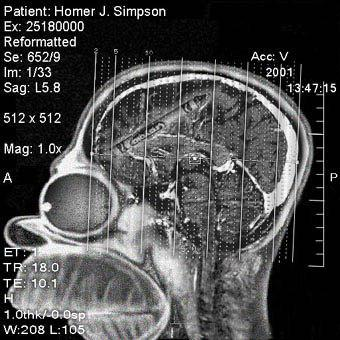
\includegraphics[scale=0.4]{img/photo_2018-07-05_14-34-53.jpg}
    \label{fig:homero}
\end{figure}
\end{frame}

\begin{frame}{PREMISAS}
\begin{itemize}
\item Nuestro “sujeto” es una imagen de $n$x$n$ pixeles discretizada en celdas de $k$x$k$ pixeles.
\item La intensidad de un pixel se asocia al tiempo que demora un rayo en atravesar ese pixel.
\item La distancia que recorre un rayo que atraviesa al sujeto es igual a la cantidad de pixeles por los que pasa.
\item En cinemática $Velocidad = \dfrac{Espacio}{Tiempo}$. En este caso la “velocidad” promedio dentro de la celda $x$ es:
\begin{displaymath}
v_{x} =\dfrac{\sum_{i=1}^{k}\sum_{j=1}^{k} I_{ij}}{k*k}
\end{displaymath}
\item Los rayos están sujetos a ruido.
\end{itemize}
\end{frame}


\begin{frame}{DESARROLLO}
\frametitle {Discretización}
\begin{itemize}
\item Utilizamos valores divisores de la dimensión de la imagen (100 x 100 pixeles).
\item En los tests de granularidad, variamos el tamaño de las celdas tomando los valores 4x4, 5x5, 10x10, 20x20, 25x25 y 50x50 pixeles.
\item A medida que se achica el tamaño de las celdas crece el tiempo de procesamiento, lo cual condicionó la elección de los parámetros.
\end{itemize}
\end{frame}


\begin{frame}
\frametitle{Recorrido de un rayo}
\begin{itemize}
\item Los rayos se consideran como rectas en el plano, caracterizados por un punto de origen y un ángulo.
\item En un vector se guardan las coordenadas de los pixeles que pertenecen a la recta y a la imagen.
\end{itemize}

\begin{figure}[H]
    \centering
    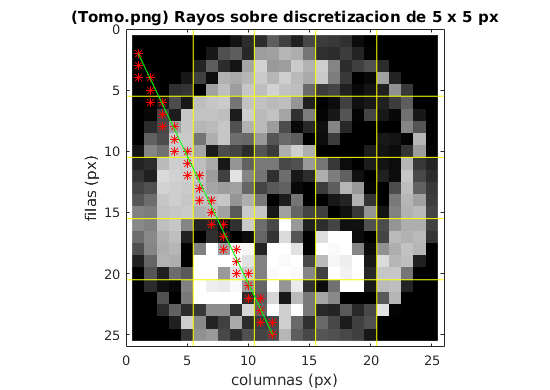
\includegraphics[scale=0.5]{img/recorridorayo.png}
    \caption{Pixeles/Celdas por la que pasa un rayo}
    \label{fig:recorridorayo}
\end{figure}
\end{frame}

\begin{frame}
\frametitle{Distancia y tiempo de recorrida de un rayo}
\begin{itemize}
\item A partir del vector de pixeles por los que pasa un rayo, se averigua a qué celda pertenece. Se suma 1 unidad por pixel. El resultado se almacena en la matriz de distancias D (una fila por rayo, una columna por celda numeradas de arriba hacia abajo y de izquierda a derecha).
\item Cada rayo toca a lo sumo $2n-1$ celdas. Se usa la estructura de matriz esparza del TP1.
\item A partir del vector de pixeles por los que pasa un rayo, se acumulan las intensidades de los mismos. Se almacenan los resultados en un vector de “tiempos” (un elemento por rayo).
\end{itemize}
$$
D = \left[
\begin{array}{cccc}
d^1_1 & d^1_2 & ... & d^1_{r^2} \\
... & ... & ... & ... \\
d^k_1 & d^k_2 & ... & d^k_{r^2} \\
... & ... & ... & ... \\
d^m_1 & d^m_2 & ... & d^m_{r^2} \\
\end{array}
\right]
,
t=\left[
\begin{array}{c}
t^1 \\
t^2 \\
... \\
t^i \\
... \\
t^{nxn} \\
\end{array}
\right]
$$
\end{frame}


% \begin{frame}
% \frametitle{Tiempo de recorrida de un rayo}
% \begin{itemize}
% \item A partir del vector de pixeles por los que pasa un rayo, se acumulan las intensidades de los mismos. Se almacenan los resultados en un vector de ''tiempos'' (un elemento por rayo).
% \end{itemize}
% \end{frame}

\begin{frame}
\frametitle{Sistema de ecuaciones}
% TODO INCLUIR MATRIZ DE ECUACIONES REALES Y DE CUADRADOS MINIMOS
% COMENTAR RELACION ENTER GRANULARIDAD, TAMAÑO DE LA MATRIZ Y CON EL TIEMPO DE PROCESAMIENTO
\par Sea $v$ es el vector de la velocidades por celda. Tenemos que:
$$
v^t=\left[
\begin{array}{c}
v_1 
v_2 
... 
v_i 
... 
v_{m} 
\end{array}
\right]
$$
\par El tiempo que tarda el rayo $k$ en atravesar al sujeto es:
$$t_{k}=\sum_{j=1}^{nxn}t^k_{j} = \sum_{j=1}^{nxn} \dfrac{d^k_j}{v_{j}} \Rightarrow Dv^{-1}=t
$$
\par Como la matriz D es rectangular con m$>>$nxn, se resuelve por cuadrados mínimos usando las ecuaciones normales:
$$
Dv^{-1}=t \Rightarrow D^tDv^{-1}=D^tt, D^tD \in R^{n^2 x n^2}
$$
\end{frame}


\begin{frame}
\frametitle{Generación de rayos}
\framesubtitle{Cantidad y ubicación de los emisores}
% COMENTAR LAS ELECCIONES FALLIDAS. 
% SI SE PUEDE GRAFICARLAS
% DESCRIBIR SELECCION DE UBICACIONES Y CANTIDAD DE EMISORES Y DE RAYOS
% MENCIONAR LOS VALORES UTILIZADOS EN LA EXPERIMENTACION

\begin{enumerate}
    \item Primeras opciones:
    \begin{itemize}
        \item Trazar rayos horizontales y verticales, formando una cuadrícula $\Rightarrow$ Filas de ceros.
        \item Trazar rayos saliendo de los cuatro vértices de la imagen en distintos direcciones para barrer los $90^{\circ}$ de cada ángulo $\Rightarrow$ Información similar, imágenes irreconocibles.
    \end{itemize}
    \item Elección final:
    \begin{itemize}
        
    \item Trazar rayos desde los cuatro laterales de la imagen.
    \item Los emisores se ubican en igual cantidad sobre los lados de la imagen.
    \item La ubicación de los emisores se selecciona aleatoriamente con distribución uniforme entre $0$ y $k$ ($k$ cantidad de pixeles por lado de la imagen.
    \item Igual cantidad de rayos en ángulos que van entre $0^{\circ}$ a $180^{\circ}$.
    \item Ángulos seleccionados aleatoriamente con distribución uniforme.
    \end{itemize}

\end{enumerate}

\end{frame}


\begin{frame}
\frametitle{Generación de rayos}
\framesubtitle{Cantidad y ubicación de los emisores}
\begin{figure}[H] 
\centering
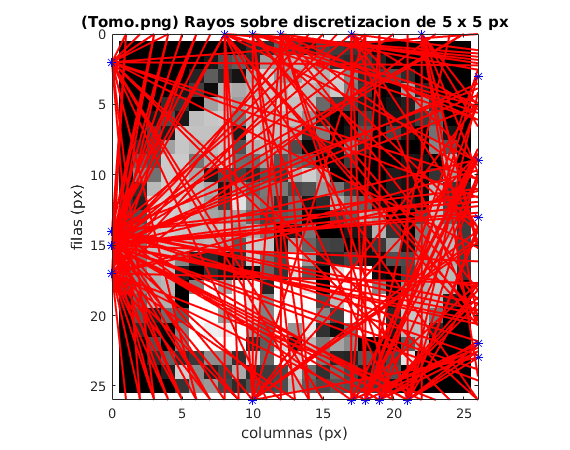
\includegraphics[scale=0.5]{img/rayos_tomo25x25px.png}
\caption{Trazado aleatorio de rayos}
\label{fig:rayos aleatorios}
\end{figure}
\end{frame}

\begin{frame}
    \frametitle{Generación de rayos}
    \framesubtitle{Casos fallidos}
    % incluir graficos e imagenes reconstruidas
    \begin{figure}[H]
        \centering
        \begin{subfigure}[h]{0.45\textwidth}
            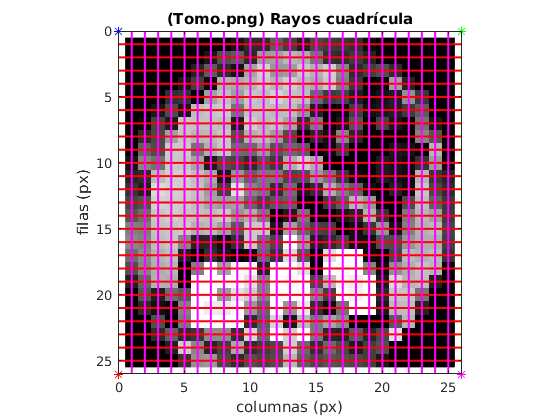
\includegraphics[width=\textwidth]{img/rayosCuadricula.png}
            \caption{Cuadrícula}
            \label{fig:rayoscuadricula}
        \end{subfigure}%
        \hfill
        \begin{subfigure}[h]{0.45\textwidth}
                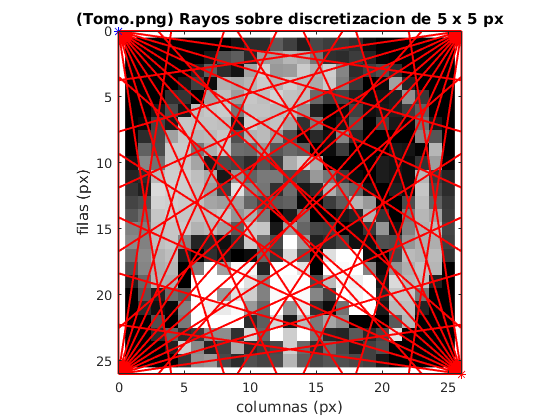
\includegraphics[width=\textwidth]{img/rayos_vertices.png}
                \caption{Desde los vértices}
                \label{fig:reconstruccion 10 px}
        \end{subfigure}
            
        \caption{Casos fallidos de distribución de emisores, sin ruido.}
    \end{figure}
\end{frame}



\begin{frame}
\frametitle{Ruido}

\begin{itemize}
\item Buscamos perturbar los datos con los que trabajamos a modo de probar qué tan robusto es nuestro sistema

\item Utilizamos ruido gaussiano con distribución $\mathcal{N}$ ~ (0, 1), el más usual. 

\item Lo aplicamos al vector $t$ que contiene los tiempos del recorrido de cada rayo.

\item ¿Por qué lo aplicamos ahora y no antes sobre la imagen original?

\end{itemize}

\end{frame}


\begin{frame}
    \frametitle{Ruido multiplicativo vs aditivo}
	\begin{itemize}
	\item Debimos decidir entre aplicar ruido aditivo (es decir, sumando una constante por un número aleatorio) o multiplicativo (proporcional al número al que se le agrega el ruido).

	\item Siendo $t_i$ un elemento del vector de tiempos, $r_i$ un elemento del vector de ruidos, $c$ una constante y $\alpha$ el parámetro de entrada:\newline $t_i + (t_i * r_i * \alpha)$ vs $t_i + (t_i * c * \alpha)$
	
	\end{itemize}

\end{frame}



\begin{frame}
    \frametitle{Ruido multiplicativo vs aditivo}
    % incluir graficos e imagenes reconstruidas
    \begin{figure}[H]
    \centering
    \begin{subfigure}[h]{0.45\textwidth}
        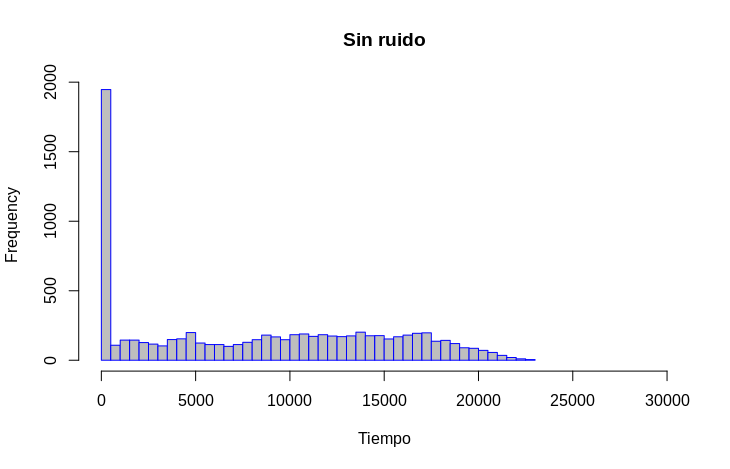
\includegraphics[width=\textwidth]{img/sinRuido.png}
        \caption{Tiempos originales}
        \label{fig:Tiempos originales}
    \end{subfigure}%
    \hfill
    \begin{subfigure}[h]{0.45\textwidth}
            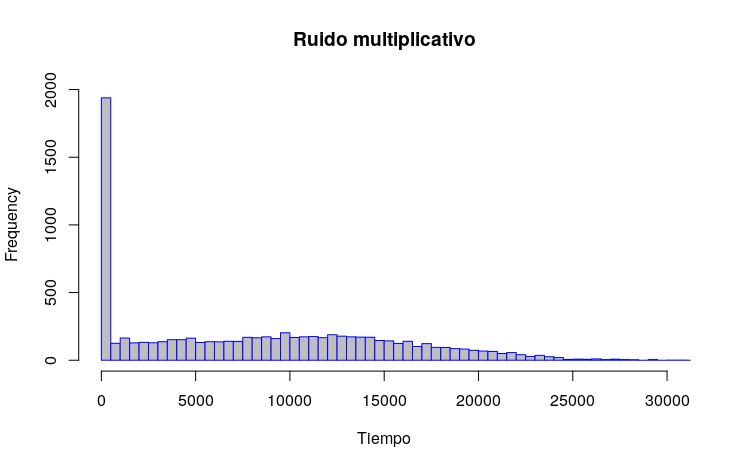
\includegraphics[width=\textwidth]{img/ruidoMultiplicativo.png}
            \caption{Tiempos con ruido multiplicativo}
            \label{fig:Tiempos con ruido multiplicativo}
        \end{subfigure}%
    \hfill
        \begin{subfigure}[h]{0.45\textwidth} 
            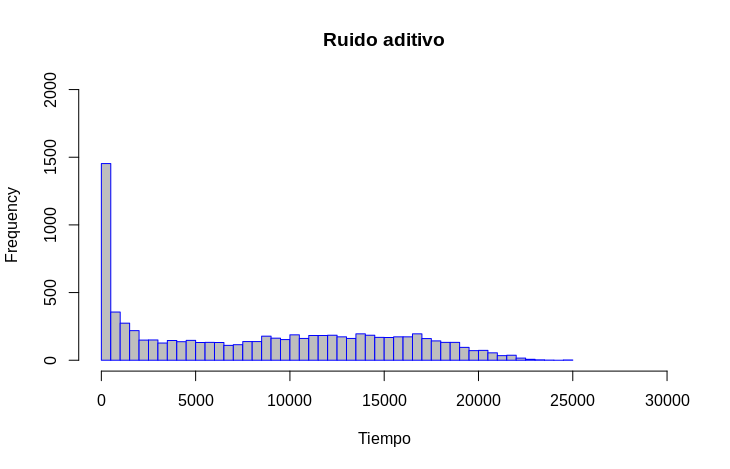
\includegraphics[width=\textwidth]{img/ruidoAditivo.png}
            \caption{Tiempos con ruido aditivo}
            \label{fig:Tiempos con ruido aditivo}
        \end{subfigure}
        
        \caption{Histogramas de tiempos de rayos comparando ruidos con el original}
    \end{figure}
\end{frame}




%%%%%%%%%%%%%%%%%%%%%%%%%%%%%%%%%%%%%%%%%%%%%%%%%%%%%%%%%%%%%%%%%%%%%%%%%%%%%%%%%%%%%%%%%%%%%%%%%%%%

\begin{frame}{RESULTADOS}
    \frametitle{Imagen original}
    % incluir graficos e imagenes reconstruidas
    \begin{figure}
    \centering
            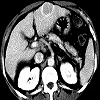
\includegraphics[scale=1]{img/tomo.png}
            \caption{Imagen original}
            \label{fig:original}
    \end{figure}
\end{frame}


\begin{frame}
\frametitle{ECM vs. ruido}
\begin{figure}
\centering
        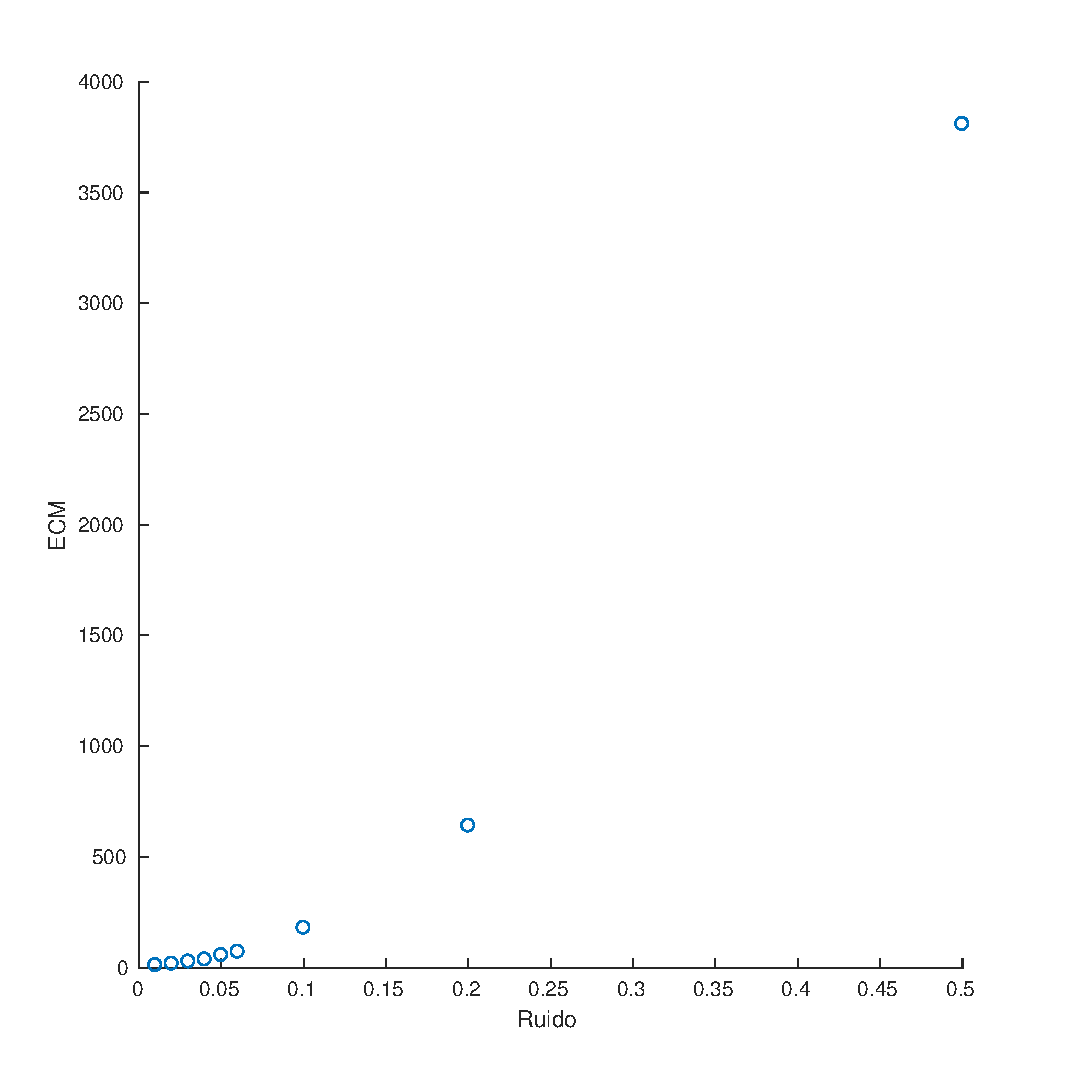
\includegraphics[scale=0.4]{img/ruido_ecm-eps-converted-to.pdf}
        \caption{Error cuadrático medio versus ruido}
        \label{fig:ECM vs ruido}
\end{figure}
\end{frame}



\begin{frame}
\frametitle{Reconstrucción variando ruido}
% comparatica de imagenes con rayos de las esquinas y de la forma que %usanmos finalmente

\begin{figure}[H]
    \centering
    \begin{subfigure}[h]{0.3\textwidth} 
        
\includegraphics[width=\textwidth]{img/tomo_ruido001.png}
        \caption{$\alpha$ = 0.001}
        \label{fig: alpha = 0.001}
    \end{subfigure}%
    \hfill
    \begin{subfigure}[h]{0.30\textwidth}
        
\includegraphics[width=\textwidth]{img/tomo_ruido005.png}
        \caption{$\alpha$ = 0.005}
        \label{fig:alpha = 0.005}
    \end{subfigure}%
    \hfill
    \begin{subfigure}[h]{0.3\textwidth} 
        
\includegraphics[width=\textwidth]{img/tomo_ruido01.png}
        \caption{$\alpha$ = 0.01}
        \label{fig: alpha = 0.01}
    \end{subfigure}


	\end{figure}
\end{frame}

    

\begin{frame}
\frametitle{ECM vs. tamaño de la celda}
% incluir graficos e imagenes reconstruidas
\begin{figure}
\centering
        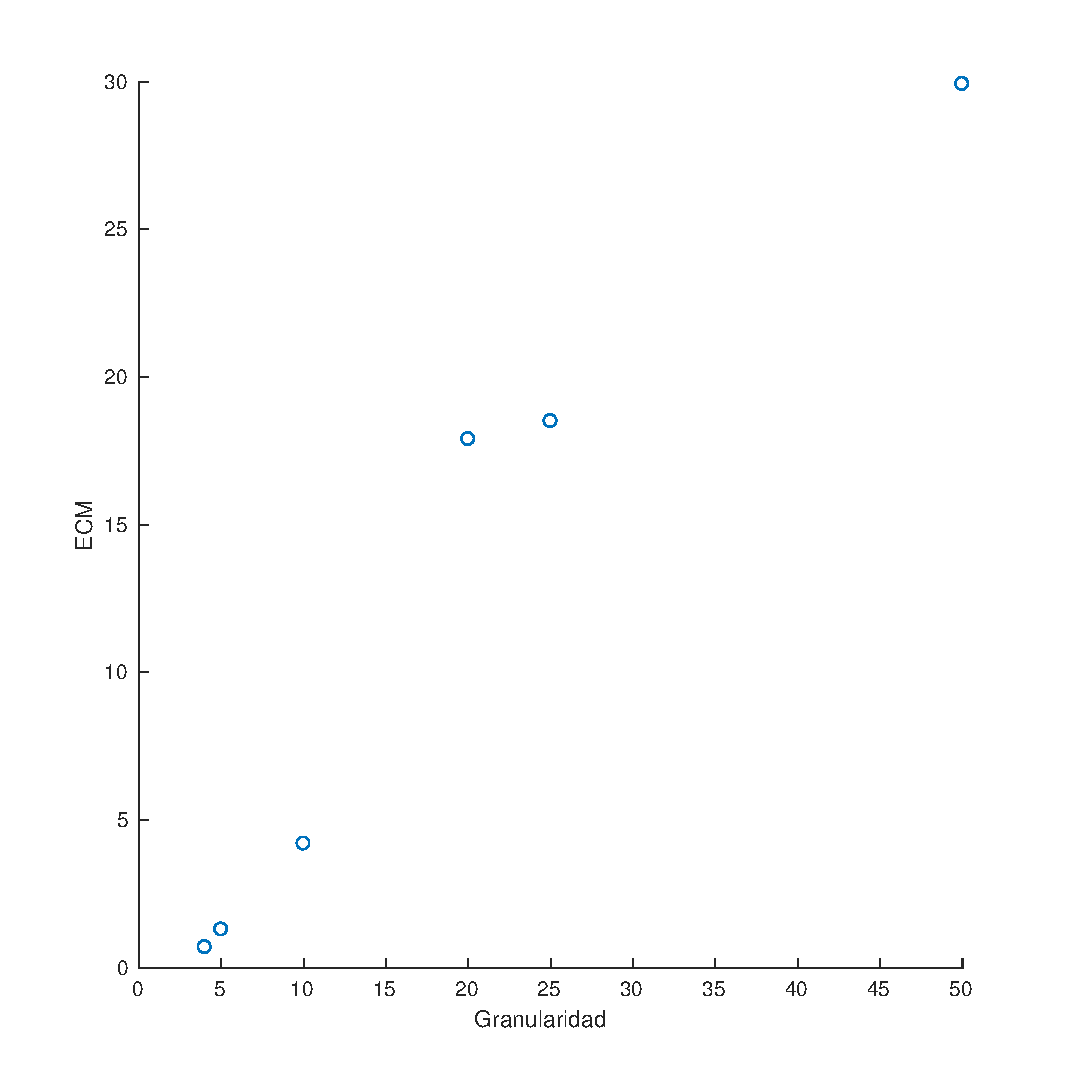
\includegraphics[scale=0.4]{img/granu_ecm-eps-converted-to.pdf}
        \caption{Error cuadrático medio versus granularidad}
        \label{fig:ECM vs granularidad}
\end{figure}
\end{frame}


\begin{frame}
    \frametitle{Reconstrucción variando granularidad}
    % incluir graficos e imagenes reconstruidas
    \begin{figure}[H]
    \centering
    \begin{subfigure}[h]{0.30\textwidth}
        
\includegraphics[width=\textwidth]{img/tomo_granu_4.png}
        \caption{4x4px por celda}
        \label{fig:reconstruccion 4 px}
    \end{subfigure}%
    \hfill
    \begin{subfigure}[h]{0.30\textwidth}
            
\includegraphics[width=\textwidth]{img/tomo_granu_10.png}
            \caption{10x10px por celda}
            \label{fig:reconstruccion 10 px}
        \end{subfigure}%
    \hfill
        \begin{subfigure}[h]{0.30\textwidth} 
            
\includegraphics[width=\textwidth]{img/tomo_granu_20.png}
            \caption{20x20px por celda}
            \label{fig:reconstruccion 20 px}
        \end{subfigure}
        
        \caption{Reconstrucción variando granularidad, sin ruido}
    \end{figure}
\end{frame}
    
\begin{frame}
\frametitle{ECM vs. cantidad de emisores}

\begin{figure}[H]
    \centering
        
            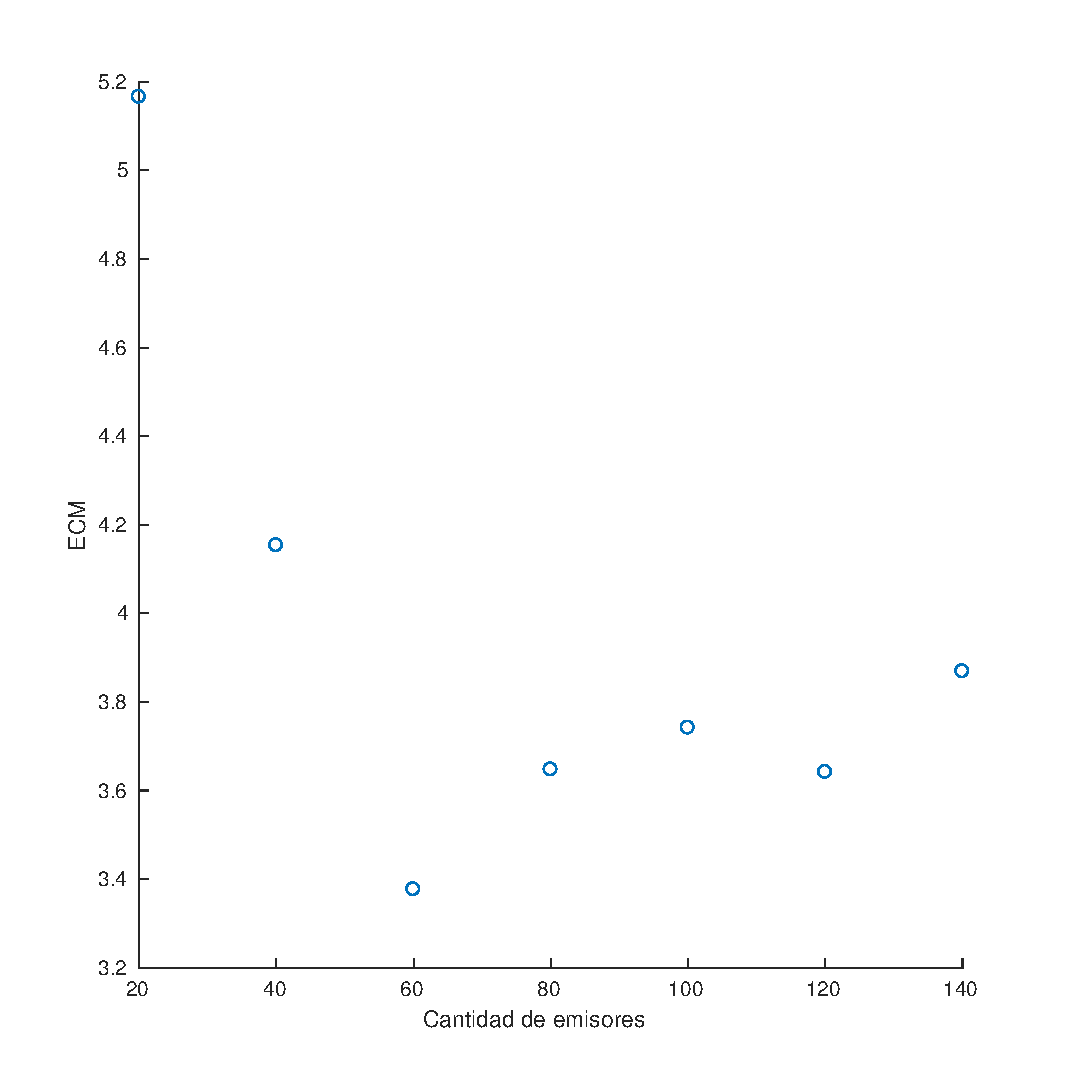
\includegraphics[scale=0.4]{img/emi_ecm-eps-converted-to.pdf}
            \caption{ECM versus cantidad de emisores}
            \label{fig:ECM versus emisores}
        
    \end{figure}
\end{frame}


\begin{frame}
    \frametitle{Reconstrucción variando cantidad de emisores}
    
    \begin{figure}[H]
        \centering
    
        \begin{subfigure}[h]{0.3\textwidth} 
            
\includegraphics[width=\textwidth]{img/tomo_emisores_20.png}
            \caption{reconstrucción 20 emisores}
            \label{fig:reconstruccion 20 emisores}
        \end{subfigure}%
        \hfill
        \begin{subfigure}[h]{0.3\textwidth}
            
\includegraphics[width=\textwidth]{img/tomo_emisores_60.png}
            \caption{reconstrucción 60 emisores}
            \label{fig:reconstruccion 60 emisores}
        \end{subfigure}%
        \hfill
        \begin{subfigure}[h]{0.3\textwidth} 
            
\includegraphics[width=\textwidth]{img/tomo_emisores_140.png}
            \caption{reconstrucción 140 emisores}
            \label{fig:reconstruccion 140 emisores}
        \end{subfigure}
        
        \caption{Reconstrucción variando cantidad de emisores, sin ruido}
    \end{figure}
\end{frame}
    


\begin{frame}
    \frametitle{ECM vs. cantidad de rayos por emisor}
    
    \begin{figure}[H]
        \centering
            
                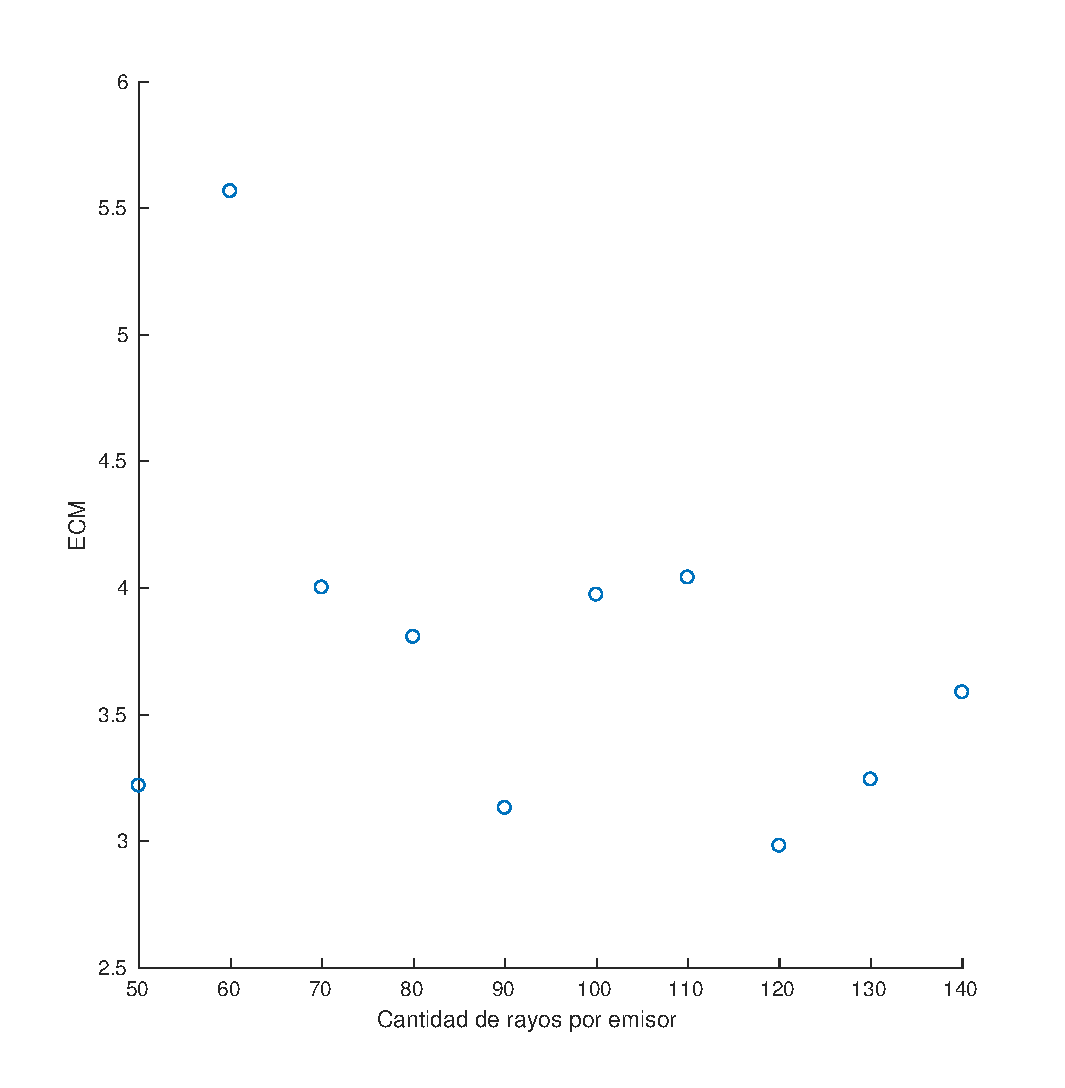
\includegraphics[scale=0.45]{img/cantrayos_ecm-eps-converted-to.pdf}
                \caption{ECM versus cantidad de rayos por emisor}
                \label{fig:ECM versus rayos por emisor}
            
        \end{figure}
\end{frame}
    


\begin{frame}
    \frametitle{Reconstrucción variando cantidad de rayos por emisor}
    
    \begin{figure}[H]
        \centering
    
        \begin{subfigure}[h]{0.3\textwidth} 
            
\includegraphics[width=\textwidth]{img/tomo_rayos_50.png}
            \caption{reconstrucción 50 rayos}
            \label{fig:reconstruccion 50 rayos}
        \end{subfigure}%
        \hfill
        \begin{subfigure}[h]{0.3\textwidth}
            
\includegraphics[width=\textwidth]{img/tomo_rayos_100.png}
            \caption{reconstrucción 100 rayos}
            \label{fig:reconstruccion 100 rayos}
        \end{subfigure}%
        \hfill
        \begin{subfigure}[h]{0.3\textwidth} 
            
\includegraphics[width=\textwidth]{img/tomo_rayos_140.png}
            \caption{reconstrucción 140 rayos}
            \label{fig:reconstruccion 140 rayos}
        \end{subfigure}
        \caption{Reconstrucción variando cantidad de rayos, sin ruido}
    \end{figure}
\end{frame}



\begin{frame}
\frametitle{Tiempo vs. granularidad}
\begin{figure}[H]
    \centering
        
            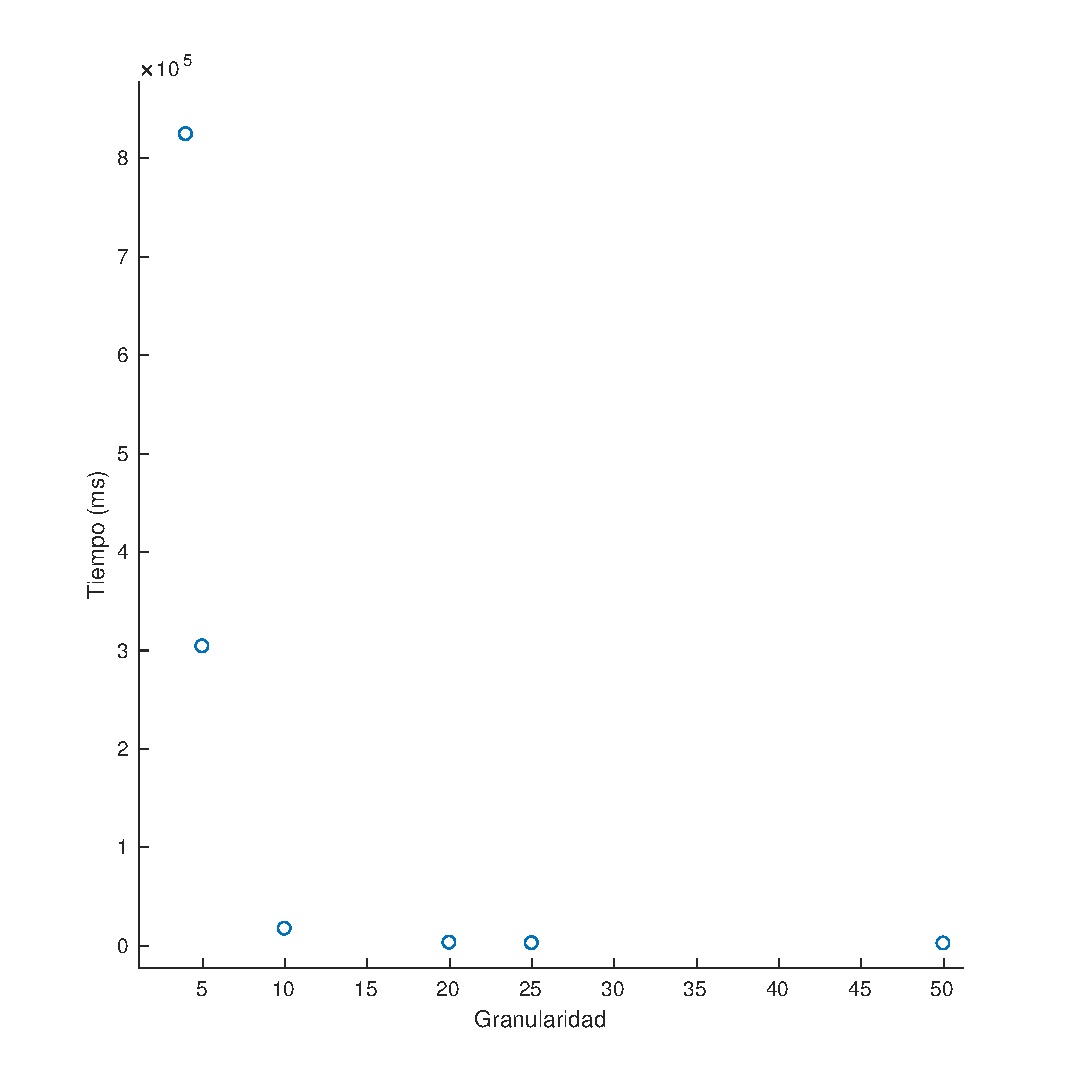
\includegraphics[scale=0.45]{img/granu_tiempo-eps-converted-to.pdf}
            \caption{Tiempo versus granularidad}
            \label{fig:tiempo versus granularidad}
        
    \end{figure}
\end{frame}


\begin{frame}
    \frametitle{Tiempo vs. cantidad de emisores}
    \begin{figure}[H]
        \centering
            
                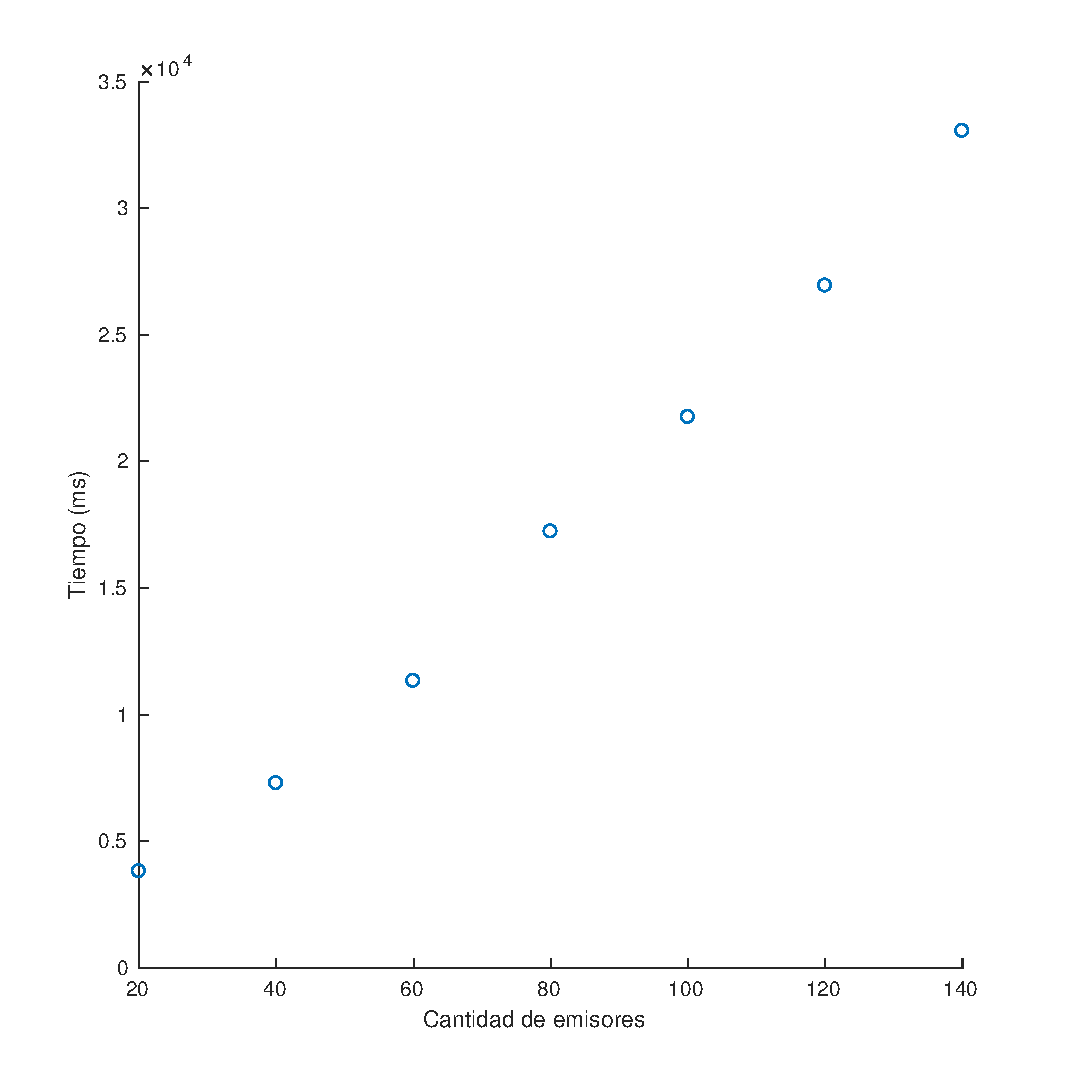
\includegraphics[scale=0.45]{img/emi_tiempo-eps-converted-to.pdf}
                \caption{Tiempo versus cantidad de emisores}
                \label{fig:tiempo versus emisores}
            
    \end{figure}
\end{frame}
    

\begin{frame}
    \frametitle{Tiempo vs. cantidad de rayos por emisor}
    \begin{figure}[H]
        \centering
            
                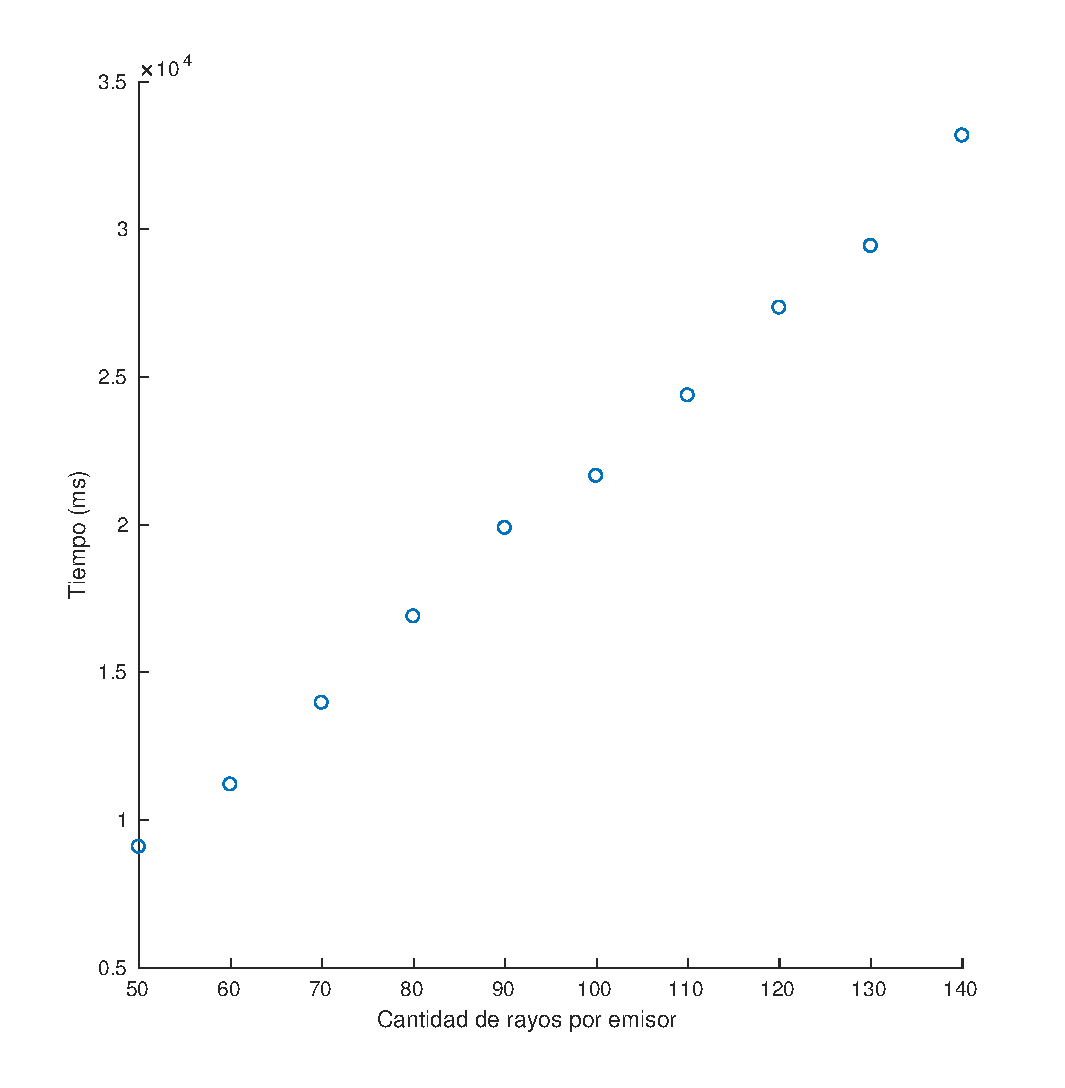
\includegraphics[scale=0.45]{img/cantrayos_tiempo-eps-converted-to.pdf}
                \caption{Tiempo versus cantidad de rayos por emisor}
                \label{fig:tiempo versus cantrayos}
            
    \end{figure}
\end{frame}


\begin{frame}
\frametitle{Comparación de resultados}
\framesubtitle{Distribución de emisores}
% comparatica de imagenes con rayos de las esquinas y de la forma que %usanmos finalmente

\begin{figure}[H]
    \centering
    \begin{subfigure}[h]{0.3\textwidth} 
        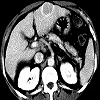
\includegraphics[width=\textwidth]{img/tomo.png}
        \caption{Original}
        \label{fig:original1}
    \end{subfigure}%
    \hfill
    \begin{subfigure}[h]{0.30\textwidth}
        
\includegraphics[width=\textwidth]{img/tomo_granu_4.png}
        \caption{Aleatoria}
        \label{fig:comp4px}
    \end{subfigure}%
    \hfill
    \begin{subfigure}[h]{0.3\textwidth} 
        
\includegraphics[width=\textwidth]{img/tomovertices.png}
        \caption{Vértices2}
        \label{fig:vertices2}
    \end{subfigure}


\end{figure}
\end{frame}


\begin{frame}{Conclusiones e ideas a futuro}

\begin{itemize}
\item Se logró realizar una reconstrucción aceptable de las imágenes.
\item La cantidad de emisores y de rayos no evidenció ser un factor determinante en la calidad de la imagen reconstruída dada la forma de trazarlos usada en este trabajo.
\item Sí lo fue la localizacion de los emisores.
\item Los tiempos de resolución del sistema de ecuaciones es un condicionante en la elección de los parámetros, principalmente la granularidad.
\item {¿Qué nos hubiera gustado mejorar?}
	\begin{itemize}
	\item Minimizar la cantidad de rayos necesarios para lograr una reconstrucción aceptable.
	\item Lograr una implementación que no utilice elementos aleatorios, esto haría que sea más plausible una implementación real de este sistema.
	\item Analizar qué otros tipos de ruido pueden presentarse en este tipo de trabajos y analizar la robustez del sistema en esos casos (por ejemplo sal y pimienta, ruido periódico, etc). 
	\end{itemize}
\end{itemize}
\end{frame}

%\begin{frame}{REFERENCIAS}
%\end{frame}


\begin{frame}
\par \begin{center}
\textbf{FIN}
\end{center}
\end{frame}



%\begin{frame}
%\tableofcontents
%\end{frame}


\end{document}

